\chapter{Introduction}\label{sec-introduction}
% (2~3 pages)
\section{Motivation}

% Introduce the background knowledge 

Classification is the problem of identifying if an observation or object belongs to a set or not, or which of several sets. It is a fundamental problem in machine learning, data mining and computer vision. With the support of the increasing capacity of computation resources and growing volume of available data, the last decades have witnessed an explosion of breakthroughs in these fields. Nowadays, classification models (classifiers) are widely adopted to solve real world tasks, including face recognition [], handwritten recognition [], sentiment analysis [] and spam filtering []. Take image classification for instance, a well-designed convolutional neural network can achieve human-level performance in a number of benchmark datasets [,]. 

% Motivation of the topic, Importance

\begin{figure}[hb]
  \centering
  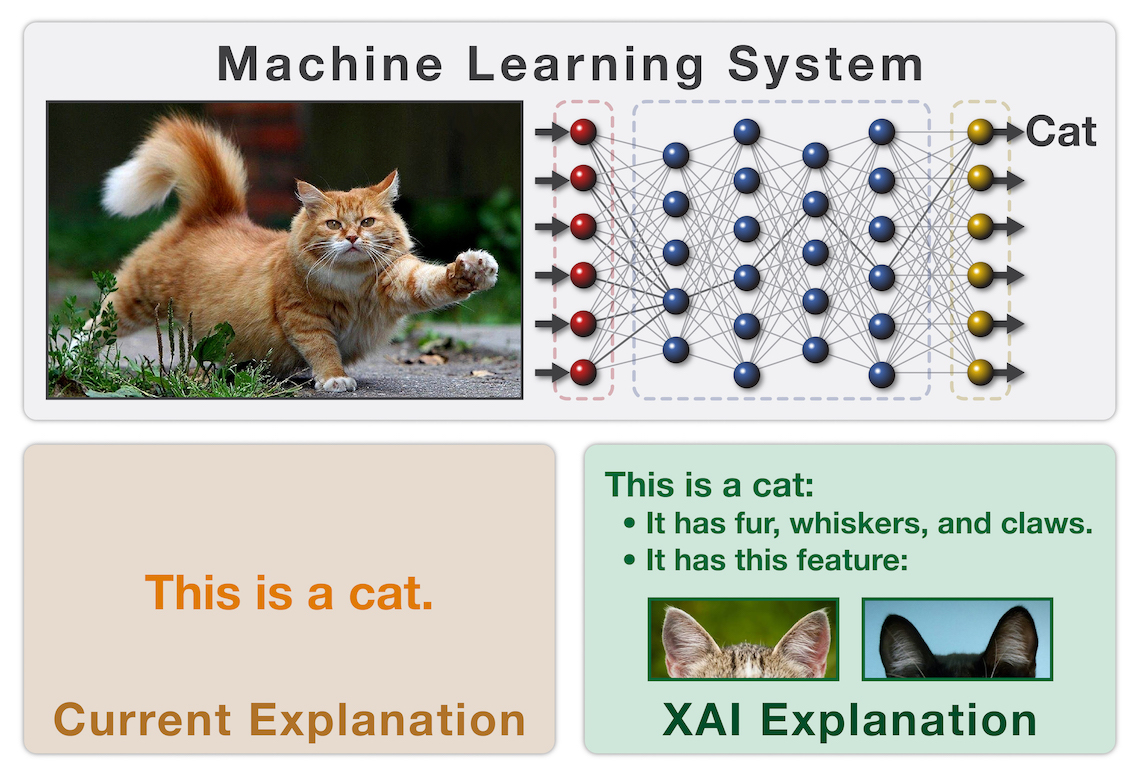
\includegraphics[width=0.6\textwidth]{figure/explain_cat}
  \caption{An illustration of an explainable image classifier \cite{darpa2017xai}.}
  \label{fig:explain-cat}
\end{figure}

Despite their promising capability, an often-overlooked aspect is the important role of humans \cite{ribeiro2016kdd}. When humans are to understand and collaborate with these autonomous systems, it is desirable if we have explanations of their outputs. For instance, a doctor using a machine classifier to assist identifying early signs of lung cancers would need to know why the classifier ``thinks'' there might be a cancer so that he/she can make a more confident diagnosis. A natural way is to provide explanations (\autoref{fig:explain-cat}). In machine learning, the term \textit{explainability} does not have a standard and generally accepted definition. In some literature, \textit{interpretability} is used instead. Generally speaking, the explainability or interpretability of an intelligent system refers to the ability to explain its reasoning \cite{doshi-velez2017interpretableml} to humans. For the sake of consistency, we use explainability as the ability to explain in this survey. Interpretability is used to refer the property of how easily a model can be understood by humans.

The research for explainable intelligent systems can be traced backed to the 1980s, when expert systems are created and proliferated \cite{clancey1981tech, neches1985tse, swartout1991expert}. These early works focused on reducing the difficulty of maintaining the complicated if-then rules by designing more explainable representations. A huge gap exists between todays state-of-the-art intelligent systems and the techniques that can make them explainable. The new challenges brought by the new generation of intelligent systems have attracted a growing research interest. DARPA launches the Explainable Artificial Intelligence (XAI) project \cite{darpa2017xai}, which aims to develop new techniques to make these systems explainable. Google Inc. initiated the People + AI Research Initiative (PAIR) \cite{google2017pair} to advance the humanistic considerations in AI. 

% The role that visualization play. Why use visualization?

Visualization, is an effective and efficient technique for communicating information and understanding complex datasets for humans. The visual system is a proxy with a very large bandwidth to human brains \cite{munzner2014visualization}. Thus, visualization can be an ideal weapon for explaining complicated classifiers for humans. Early related research can be traced back to the software and algorithm visualization for computer science education in the 1980s and 1990s \cite{brown1987aa,stasko1990aa,price1992taxonomy}. Visualization, especially interactive visualization, was proved to be very effective in facilitating people's understanding of complex softwares and algorithms.
Few research has been done to visualize the increasingly complicated classifiers, which are actually algorithms learned from the data. It is not until recently that visualization was popularized as a media for understanding classification models, especially for image classifiers \cite{simonyan14saliency,zeiler2014eccv,bach15plos,zintgraf17visualize}. However, these methods have limited applications to neural networks for image data. There is also a lack of a unified and convenient evaluation method for the generated visualizations. 

\section{Challenges}

The need for visually explaining classifiers is actually a result of the successes and advances of AI. The major challenges of visually explaining classifiers results from the complexity of the model and data, and the limits of humans.

First, it is challenging to explain complex classification models both concisely and precisely. The best-performing classifiers (e.g., neural networks) are becoming increasingly complex, in terms of the number of parameters and operations they employed, which makes them difficult to be explained. A convolutional network typically employs thousands of neurons and millions of parameters. A random forest used for classification may employ hundreds of decision trees, each contains hundreds of nodes. Sampling a small number of parameters/neurons/nodes to explain might be easier to understand for humans, but it brings risks of misunderstanding as well. The variety of model architectures also increases the difficulty for a explanation framework for classifiers to be effective and general at the same time. 

Another challenge is the volume and variety of the data used for training the classifiers. To explain a classifier, a most common strategy is to trace back to the input data. Which part of the input data contributes to the prediction? How the model behaves on this subset of data? Some explanation methods require computations over the whole training data, which may become impractical if the data set is very large. Different data types may require different forms of visual explanation. Image data are readily interpretable, but how to effectively explain classifiers on categorical, text and speech data is still a problem.

These challenges are, to some extent, due to the compromise with the limits of humans' cognition ability. If humans can make sense of the meaning of thousands of parameters and complex model structures by merely looking at the raw data or code, there is no needs struggling on how to better visualize them. There is already some studies discussing the structure, function and effectiveness of explanations in cognitive science. However, it is still unclear how we can effectively evaluate the quality of an explanation, and the load that its visual representations exert to humans.

% Summarize the research challenges of the topic

\section{Overview}

This survey mainly focuses on how visualization techniques can be used to support explainable classifiers. In \autoref{sec-explainable-classifier}, we first introduce the definition of classification and classifiers, and the concept of explainable classifiers. Two major research directions towards more explainable classifiers are identified: designing classifiers that are readily interpretable, and methods that generate explanations for a classifier without modifying the model. In \autoref{sec-visualization}, we first articulate the life circle of a classifier into different stages, i.e., the recursive procedures of data collection and processing, model development and testing, and operations and maintenance. Then, we illustrate how visualization can be applied at different stages to provide explainability of classifiers. Based on the specified life cycle, we categorize the surveyed literature and discuss the challenges and opportunities for future research in visualization for explainable classifiers.

\newpage
